\chapter{Préparation du travail et ordre des opérations}\label{ch:preparation}

\section{Préparation du véhicule}
Suivez la séquence ci-dessous pour remplacer le combiné d'origine par un tableau Digifiz~:
\begin{enumerate}
    \item Retirez les garnitures plastiques recouvrant les pédales et la partie inférieure du tableau de bord pour mettre à nu le bloc instruments d'usine.
    \item Débranchez la batterie du véhicule.
    \item Déconnectez le faisceau du combiné d'origine.
    \item Désaccouplez le câble de compteur mécanique, s'il est présent.
    \item Dévissez le combiné de ses supports et retirez-le délicatement du véhicule.
    \item Faites cheminer les faisceaux de température et de capteur de vitesse fournis selon les besoins.
    \item Installez le tableau Digifiz dans les glissières de support et fixez-le avec les vis.
    \item Pour \ReplicaNextLong{}, installez les capteurs Volkswagen MFA (ou équivalents) et amenez leurs fils vers les connecteurs CE~1/CE~2.
    \item Sur les modèles \texttt{GACS}/\texttt{GARS}/\texttt{DARS}/\texttt{DACS}, raccordez manuellement les fils étiquetés \texttt{MFA\_MODE}, \texttt{MFA\_RESET}, \texttt{MFA\_BLOCK} et frein à main si le faisceau véhicule ne possède pas ces contacts. La seconde génération \ReplicaNextShort{} relie ces signaux en interne par défaut.
    \item Branchez les faisceaux sur le tableau.
    \item Montez le capteur de vitesse électronique ou reconnectez le câble mécanique.
    \item Reposez les garnitures du tableau de bord et le cache-pédales dans l'ordre inverse.
\end{enumerate}

\section{Utilisation du tableau}
\begin{itemize}
    \item Le tableau s'alimente automatiquement avec le contact. L'interrupteur des feux de position commande le rétroéclairage.
    \item Au démarrage, toute l'échelle de vitesse s'allume pendant que les diagnostics internes stabilisent le modèle de régime ; l'affichage se fixe ensuite sur le ralenti courant.
    \item Dès que le véhicule se met en mouvement, le système indique les paramètres listés au \Cref{ch:technical-specs}.
\end{itemize}

\subsection{Fonctions MFA}
Six pages MFA sont disponibles~:
\begin{enumerate}
    \item Durée de fonctionnement journalière.
    \item Distance parcourue.
    \item Consommation de carburant (non implémentée sur la première révision Replica).
    \item Vitesse moyenne (affichée multipliée par dix).
    \item Température d'huile moteur (faisceau externe requis).
    \item Température ambiante (faisceau externe requis).
\end{enumerate}
Sur les tableaux \ReplicaGenOneShort{}, un point tactile capacitif derrière le logo VW fait défiler les pages ; \ReplicaNextShort{} utilise un commutateur de colonne externe. Les durées de contact se comportent ainsi~:
\begin{itemize}
    \item Appui court (\(<1\)~s)~: passe à la fonction MFA suivante.
    \item Appui moyen (1--3~s en l'absence de commutateur de colonne)~: change de bloc mémoire MFA ; la modification est indiquée à l'écran.
    \item Appui long (3--7~s)~: réinitialise la fonction MFA active (consommation, distance, durée et vitesse moyenne).
\end{itemize}

\subsection{Rétroéclairage et disposition des voyants}
Le tableau \ReplicaGenOneShort{} propose une molette de luminosité manuelle au-dessus de l'interrupteur des feux de stationnement ; \ReplicaNextShort{} s'appuie sur un réglage automatique piloté par photodiode. Des dérogations manuelles peuvent être configurées via les interfaces de maintenance décrites aux \Cref{ch:replica-setup,ch:replica-next-setup}.

La disposition de la barre horizontale de voyants et la légende à l'écran sont illustrées à l'\autoref{fig:indicator-layout}.

\begin{figure}[htbp]
    \centering
    \begin{subfigure}{0.48\textwidth}
        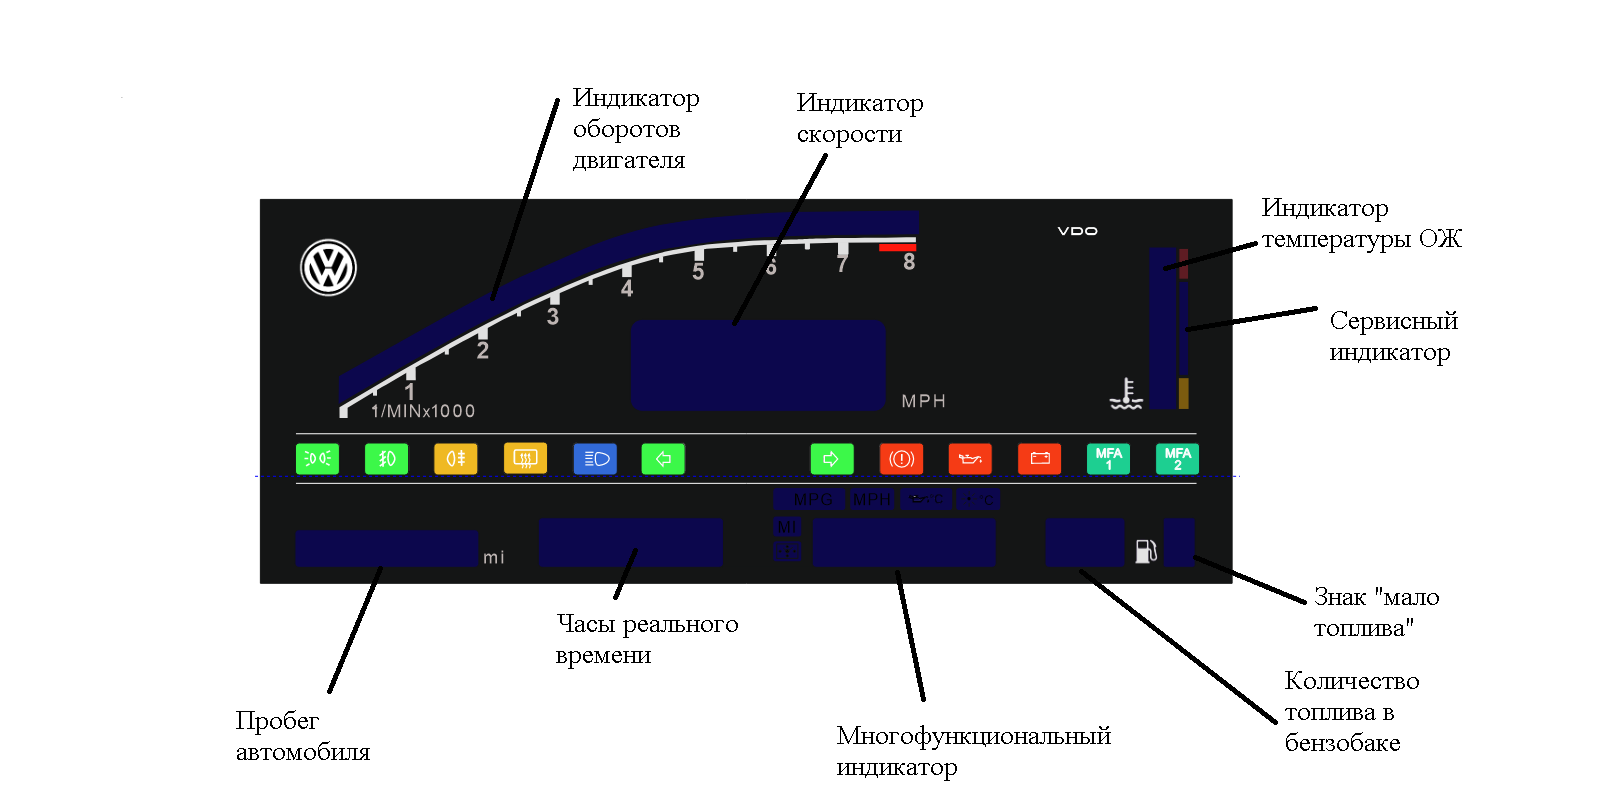
\includegraphics[width=\linewidth]{digifiz_manual/image017.png}
        \caption{Disposition des voyants affichée lors de l'auto-test.}
    \end{subfigure}\hfill
    \begin{subfigure}{0.48\textwidth}
        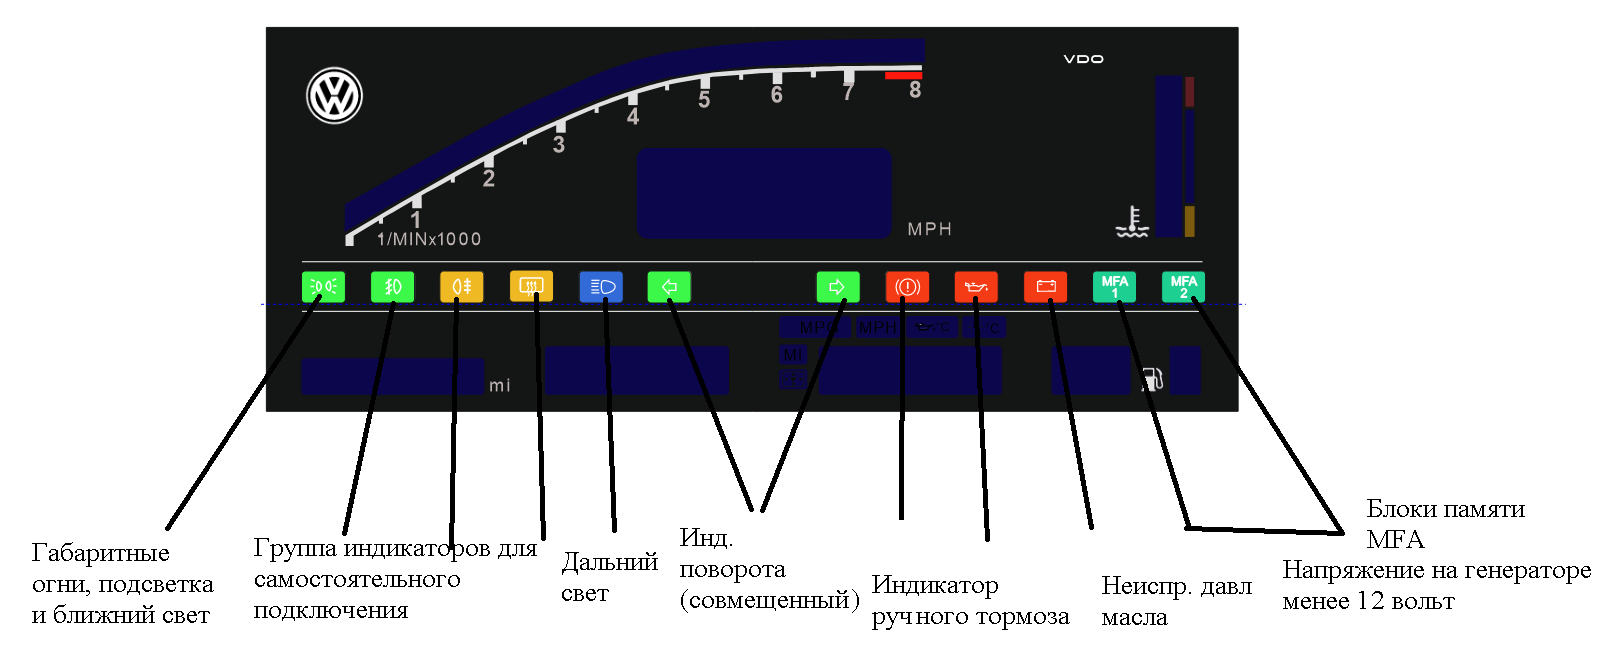
\includegraphics[width=\linewidth]{digifiz_manual/image018.png}
        \caption{Légende de la barre horizontale de voyants.}
    \end{subfigure}
    \caption{Schéma d'indication du combiné.}
    \label{fig:indicator-layout}
\end{figure}

\subsection{Interfaces de configuration}
\begin{itemize}
    \item Les unités \ReplicaGenOne{} classiques intègrent un module Bluetooth 2.0 (ou compatible BLE). Installez l'application \emph{Serial Bluetooth Terminal} depuis Google Play, associez-la au tableau et envoyez les commandes depuis la console. Les appareils Apple iOS ne peuvent pas se connecter à ce module.
    \item \ReplicaNextShort{} expose un point d'accès Wi-Fi embarqué et un portail de configuration décrits au \Cref{ch:replica-next-setup}. Désactivez les données mobiles pendant la connexion pour que le portail captif se charge correctement.
\end{itemize}
Les deux générations peuvent également être alimentées et configurées sur établi via l'interface de programmation USBasp.
